
\documentclass{article}

\usepackage{arxiv}
\usepackage{graphicx}

\usepackage[utf8]{inputenc} % allow utf-8 input
\usepackage[T1]{fontenc} % use 8-bit T1 fonts
\usepackage{hyperref} % hyperlinks
\usepackage{url} % simple URL typesetting
\usepackage{booktabs} % professional-quality tables
\usepackage{amsfonts} % blackboard math symbols
\usepackage{nicefrac} % compact symbols for 1/2, etc.
\usepackage{microtype} % microtypography
\usepackage{lipsum}
\usepackage{float}


\title{Review of current ultrasound hardware considerations, designs, and processing opportunities}





\author{
 Luc Jonveaux\thanks{Lead of the un0rick.cc project } \\
 Open-source hobbyist \\
 Milly le Meugon, FR\\
 \texttt{kelu124@gmail.com} \\
 \And
 Carla Schloh \\
 Fraunhofer MEVIS\\
 Institute for Digital Medicine\\
 Bremen, DE\\
 \texttt{ carla.schloh@yahoo.de} \\
\And
 William Meng \\
Columbia University \\
 New York, US\\
 \texttt{ wlm2117@columbia.edu} \\
 %% examples of more authors
 \And
 Jorge Arija \\
MicroComp \\
 Bilbao, ES\\
 \texttt{ jarija@microcomp.es} \\
   \And
 Jean Rintoul \\
Mindseye Biomedical \\
 London, UK\\
 \texttt{ jean@mindseyebiomedical.com} \\
 }


\begin{document}
\maketitle

\begin{abstract}

Ultrasound is one of the most widely used imaging tools for non-destructive testing (NDT) and non-invasive medical diagnosis.
Since its beginnings in the 1970s, ultrasound has been an ongoing field of research,
with innovations such as new sensors, signal processing, and hardware development. After more than fifty years, the field still presents active developments, renewed by electronics and digital equipment improvements over the last years.

However, within the realm of open-source equipment, the field remains under-researched in terms of experimental hardware. An open, flexible and cost-efficient platform is still needed for many medical and testing basic applications to support the efforts of the researchers, makers and device developers, to accelerate ultrasound research and development.

The aim of this review is to identify literature that is relevant for understanding, designing and operating a simple single-channel ultrasound device, and to capture this body of knowledge and make it accessible to ultrasound system designers. It also aims at presenting current ultrasound research focus points to introduce the reader to trends of interest.

We try to capture design and use considerations from older and newer designs, but also with high-end, and multi-channel systems. We have covered both NDT and medical applications, starting with a review of the context, following on the review of existing architectures and analog buildings blocks, then on digital options available to support and complement the hardware aspects.

This body of knowledge was used for designing two relatively simple open hardware designs.



\end{abstract}


% keywords can be removed
\keywords{ultrasound \and hardware \and open-source \and frugal device \and imaging \and single-element \and modular design}

% this table is to be removed before submission
%\tableofcontents

\newpage


\section{An introduction to open ultrasound hardware}

\subsection{A renewed interest in ultrasound}

Ultrasound has been a developing field for medical imaging and non-destructive testing and exploration (NDT/NDE) that bloomed the 1950s. Although ultrasound is today a relatively mature technology, it remains an active field of study, and  there are aspects that have yet to be further explored, such as CMUT sensors and compressed sensing \cite{kruizinga_compressive_2017, liebgott_compressive_2012}, which have the potential to revolutionize ultrasound imaging, leading to three figure dollar price tag devices.

With this in mind, it makes sense to build an affordable and extensible platform for ultrasound research that leverages advances in low-cost computing in order to offload functions which previously required dedicated hardware.

Ultrasound imaging has numerous advantages over other widely-used imaging modalities, such as computer tomography (CT) or magnetic resonance tomography (MRI), particularly because it is deemed safe and affordable. As a result of these characteristics \cite{kurjak_use_1986}, it has become an important tool in medical care. The World Health Organisation \cite{who_future_1985} recognises and stresses the advantages of using ultrasound in medically under-served regions such as low- and middle-income countries where other technology is simply not affordable or the infrastructure non-existent, now focusing in particular smaller systems \cite{kjeken_systematic_2011}.
 


\subsection{Open-source ultrasound hardware}

Open-hardware lowers barriers to product research \cite{pandey_open_2019}, having a full design under an open-source license provides access for all researchers to contribute to and improve a design. This in turn creates the potential for rapid spread of the design, customisation for specific uses, and ad-hoc modification. The existence of an open design means that a higher number of contributors can inspect and improve it. Open source hardware can be a disruptive tool on the medical device market. Shorter development cycles, even for hardware, with open source permit rapid iterations of a product, for which the economic impacts can be significant \cite{pearce_quantifying_2015, pearce_return_2016, moritz_economic_2019, winter_open_2019}.

Because they are medical hardware and devices, it is essential to ensure that these tools have the functions they are designed to have: quality and medical certification are critical. As such, certification of open-hardware designs is a challenge that needs to be tackled, starting, for example, from a CE marking perspective. Alternatively, it funding certification through crowd-funding approaches has been proposed \cite{de_maria_safe_2018}. According to the WHO, 70–90 percent of all medical devices donated to the developing world do not function as intended, and 20 percent are not used due to poor documentation and inadequate training on the use of the device \cite{niezen_open-source_2016}. Since their hardware and software architecture are not public knowledge, it is impossible for users to access and repair them. Using open-source products, this problem could be avoided, in contrast, support could be provided online detailing how to repair these systems \cite{gibney_open-hardware_2016}.

\section{Review of ultrasound usage}

\subsection{The main ultrasound imaging modes}

With the exception of Doppler imaging, ultrasound imaging is based on the "pulse-echo" principle, which relies on the dual receiver-transmitter function of a piezoelectric transducer. The two main modes commonly found in ultrasound equipment are:

\textbf{\textit{A-Mode}}, or amplitude mode, is used to display the direct amplitude of echoes received as a function of time and creates one-dimensional images.

\textbf{\textit{B-Mode}}: In B-Mode ultrasound, the most common form of ultrasound imaging, a 2D image is produced. It displays the envelope of the recorded symbols, typically in grey-value representation on a 2D map where every value is assigned a different shade of grey. The higher the intensity of the echo, the brighter the reflection interface in the reconstructed image. This is the widely known sonogram used to examine babies in utero.

Other modes, such as M-Mode, C-Mode, and Doppler  extend the previously discussed modes, but are beyond the scope of simple imaging methods.

\textbf{\textit{Tomography}}: though less common than the previously discussed uses, ultrasound can be used in tomography for imaging soft tissue \cite{zhang_design_2015, duric_detection_2007, wen_design_2019, ashfaq_new_2004}, in this application, a transducer or array of transducers is used to measure acoustic impedance at different angles and an image is reconstructed using back-projection or related finite element techniques. The same acoustic impedance methods used in tomography have also been used to recreate images with high temporal and spatial resolution in recent research on plane wave acoustic imaging\cite{Rabut2019,Warner2013}. Recent acoustoelectric imaging systems are able to combine the acoustic image with a current-source density image, suggesting promising novel applications in electrophysiology\cite{Xi2009, Qin2017}. New computing techniques for full wave imaging have also the opened door to better imaging \cite{guasch_full-waveform_2020, rymarczyk_logistic_2019}. 

\subsection{A wealth of applications}

\textbf{\textit{Overall imaging}}: although it is relatively simple and does not enable 2D imaging, A-mode enables 
measurements for examinations such as para-nasal sinuses, trans-skull fluid detection, sinus pathology, skeletal muscle detection in the wrist extension \cite{noauthor_wrist_nodate}, measurement of the artery lumen diameter \cite{hu_design_2011, zhang_multi-channel_2017, shomaji_early_2019}, bone porosity \cite{wahab_design_2016, fontes-pereira_monitoring_2018, grasel_characterization_2017} and ophthalmology assessments \cite{carotenuto_very_2004}.

Ultrasound can be used for \textbf{\textit{Vascular assessments}}, to measure the diameter and the blood pulse speed traveling through the radial artery \cite{worthing_using_2016}, which then can be used to track changes in blood pressure at various points on the human body. Other \textbf{\textit{body monitoring}} uses can include artery stiffness measurements \cite{joseph_technical_2015, joseph_artsenstouch_2015, seo_non-invasive_2018}, monitoring bone density \cite{wahab_design_2016, fontes-pereira_monitoring_2018},tissue assessment \cite{keyes_electrical_2017}, including muscle evolution \cite{brausch_towards_2019} for example quantifying neuro-muscular disease progression \cite{zhang_design_2015}, both using A-mode and B-mode imaging. \textbf{\textit{Body composition assessment}} is another application of A-mode imaging \cite{wagner_validity_2016, martins_-scan_2017}. The measurement of \textbf{\textit{bladder volumes}} is also a standard medical use \cite{kuru_feasibility_2019}. Another use can be providing \textbf{\textit{biofeedback}}, as it has been shown that ultrasound imaging enables the tracking of muscle movements \cite{sikdar_novel_2014} and follow-up of biofeedback in stroke reeducation \cite{sosnowska_training_2019}. Last but not least, ultrasound has also been used in \textbf{\textit{tracking body movements}}, for example, tracking obstructive sleep apnea (OSA) \cite{weng_fpga-based_2015}, breathing patterns \cite{shahshahani_ultrasound_2018}, and heart muscle behavior \cite{nguyen_estimating_2019}.

Other interesting uses include the development of \textbf{\textit{ultrasound capsules}}, typically swallowable devices, which enable endoscopy imaging using high frequency ultrasound by fitting the hardware into a 10mm diameter by 30 mm long capsule \cite{cox_ultrasound_2017, wang_development_2017}. Capsules promise further development, and their architecture can be a source of inspiration \cite{lee_towards_2014, memon_capsule_2016, lay_progress_2016, lay_-vivo_2018}. \textbf{\textit{Wearable devices}} are also gaining momentum due to the miniaturisation trend in components and sensors \cite{basak_wearable_2013}. This is also seen in \textbf{\textit{neuromodulation}} \cite{pashaei_flexible_2020} applications, where, interestingly, ultrasound can be used both to power devices and communicate with them \cite{johnson_stimdust_2018, seo_wireless_2016, santagati_design_2020}, and even to stream video \cite{kou_real-time_2020}.

Ultrasound can also be used for \textbf{\textit{nondestructive testing (NDT)}} or nondestructive examination (NDE)  \cite{duncan_real-time_1990,noauthor_integration_nodate}, for quality or integrity control of mechanical elements. \cite{fritsch_full_nodate} presents a very interesting design for single-element FPGA-based NDE design, migrating traditionally analog functions, like filtering and envelope extraction, to the digital domain developed by others  \cite{triger_modular_2008, shrisha_fpga_2018, rodriguez-olivares_improvement_2018}, as we will see below. 


\subsection{Minimal specifications for a B-Mode device}

As a reference for the next sections, reviewed literature offer a view of a minimal B-mode imaging system, in particular thanks to \cite{kurjak_use_1986} who laid out the basic specifications for a general purpose ultrasound scanner. This basic, minimal specification set can allow designers to frame the development of their own systems, captured in precursor portable devices such as with the Sonovisor \cite{zeiss_sonovisor_1962}. From this, as well as the previously reviewed designed, it is deemed necessary to build a basic ultrasound scanner to:

\begin{itemize}
\item produce B-mode images, which translates as a device having linear- and convex- type scan-heads
\item image at least 3.5MHz -- extendable to 5MHz
\item image of human tissues requires at least 50dB of SNR \cite{attarzadeh_low-power_2017} translating with a 9-bit ADC 
\item images should be displayed on a reconstructed 512 x 512 image, on 4 bits.
\item images should go to a depth of 18cm, meaning 240us of acquisition, in line with a 512 pixel-deep image considering a single-element resolution. 
\item viewing angle of 40 degrees or more, which indicates that 128 lines per image should be sufficient.
\item image should be refreshed at 5 to 10fps.
\end{itemize}

\newpage
\section{Considerations leading to the design of the system architecture}

The following section provides an overview of the available hardware architectures for ultrasound devices, based on an earlier similar review \cite{jonveaux_arduino-like_2017} or with more complex designs \cite{roman_open-source_2019}.

\subsection{Sourcing information }

Apart from the projects aimed at developing open-source ultrasound hardware described in this article  \cite{roman_open-source_2019, luc_jonveaux_un0rick_2019}, several sources can be consulted to inform the design stage. The main one has been a scientific literature review, offering insights in terms of research devices designs and major technology evolution over the years, reflecting both medical and ndt state of the art.

A secondary source of information has been patents, as made publicly available on the Internet. 

Teardowns of medical devices available online have also provided information about the state of the art in terms of hardware architecture. However, investigations of this kind are relatively infrequent, as this activity requires that researchers have both specific skills and interest in dismantling expensive equipment. Refurbished equipment from the 80s and 90s, such as mechanical probes, can be an affordable source of sensors, in addition to providing useful ideas and concept  from a design perspective.  

Chip makers can be considered actors in the diffusion of knowledge and know-how \cite{brunner_how_2002, xu_challenges_2010}, as they are major producers of concept and design notes. Chip makers also provide guidance on designs \cite{ching_chu_designing_nodate}, but integrating these components can be challenging. For example, datasheets may be incomplete or erroneous. To support the use of their circuits, chip makers have also proposed evaluation kits -- but these may be overly complex for a simple hobbyist, in addition to being somewhat expensive.

Finally, equipment suppliers provide researchers with similar equipment, making it possible to better understand the required functionalities. They include:
\begin{itemize}
\item
Verasonics \cite{peyton_front-end_2017, george_portable_2018, kang_new_2017, hager_ultralight:_2017} 
\item Lecoeur Electronique \cite{lecoeur_bluetooth_nodate, tortoli_ula-op:_2009, zhang_toward_2018, al-aufi_thin_2019}
\item Ultratek \cite{veenstra_generating_nodate, perez-sanchez_numerical_2020, chen_ultrasound_2016, wang_preliminary_2019}
\item Optel \cite{ scholle_pulse_2018, ratajski_application_2017, nowak_evaluation_2020, karjalainen_multi-site_2012},
\item Eurosonic \cite{jin_optimization_2017, mostavi_application_2017, ranachowski_mechanical_2020, vadalma_smartphone_2020}, 
\item Biosono \cite{biosono_sonolab_nodate} 
\item or  the Fraunhofer Institute \cite{zimmermann_highly_2019, zimmermann_miniaturized_2018, zimmermann_high_2018} 
\end{itemize}

Other suppliers have made smaller contributions to the literature \cite{ozdemir_remote_2018}, such as Socomate \cite{gil-alba_morphological_2019}, MATEC TB-1000 \cite{kielczynski_thermophysical_2017} JSR Ultrasonics \cite{cramer_ultrasonic_2015}, or high-speed Dr Hillger's USPC \cite{hillger_high_2016}. 


\subsection{Functional blocks composing ultrasound systems}

The functions required in a single-element ultrasound pulse-echo system (shown in Figure \ref{fig:BlockDiagramme}) are relatively standard and are well described in the literature \cite{murtaza_ali_signal_2008}.

\begin{figure}[H]
 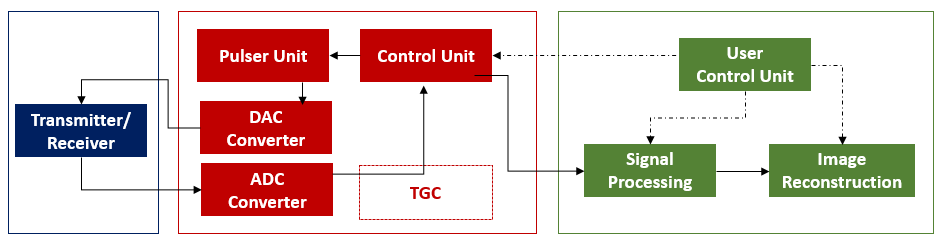
\includegraphics[width=\linewidth]{images/Blockdiagramme.PNG}
 \caption{Block diagram of a single-element ultrasound system showing the functions needed for a simple ultrasound device}.
 \label{fig:BlockDiagramme}
\end{figure}
These blocks are used to create the pulse-echo pattern that ultimately creates an ultrasound image, be in in A-mode or B-mode.


\subsection{Earlier works on simple hardware architectures for ultrasound systems}

The first reviewed research setup appears to date back to 1993 \cite{jensen_deconvolution_1993}, in which a Bruel \& Kjaer, BK Type 1846 was modified to accept research equipment.
Since early 2000, several groups of researchers have worked on designing and implementing research-friendly equipment. Most of these designs are for multi-channel devices \cite{boni_ula-op_2016, boni_reconfigurable_2012, boni_ultrasound_2018, qiu_flexible_2012, levesque_architecture_2011}, but other authors have considered single-element designs, such as \cite{carotenuto_fast_2005} and \cite{richard_low-cost_2008}. An interesting modular design was proposed in \cite{wall_high-speed_2010} which has a motherboard connected to the device. More recently, \cite{taylor_development_2017} also used a beagle bone device. \cite{jonveaux_arduino-like_2017} proposed an Arduino-like approach to functional blocks, balanced by SNR and cost impacts, which may have inspired further designs \cite{golabek_construction_2019}.

\subsection{State of the art and review of the ultrasound hardware designs}

\subsubsection{Design sources for the state of the art review}

A summary of the literature with respect to ultrasound system design, based on a review of components used, is presented in the table below. High-end systems were considered in this review, as it is possible to exploit aspects of their design approach for use on simpler platforms. 

% Please add the following required packages to your document preamble:
% \usepackage{booktabs}
 
\begin{table}[H]
\centering
\begin{tabular}{l|c|c|c|c|c|c}
\textbf{Reference}                               & \textbf{Elements} & \textbf{Voltage} & \textbf{Msps} & \textbf{Res} & \textbf{AFE-TGC}    & \textbf{Year}   \\ \hline
\cite{ahn_smartphone-based_2015}    & 16          & 70V     & 40   & 10   & AFE5808 & 2015 \\
\cite{assef_compact_2014}      & 128         & 100 Vpp & 50   & 12   & AFE5805 & 2014 \\
\cite{assef_design_2012}       & 128         & 100 Vpp & 50   & 12   & AFE5805 & 2012 \\
\cite{assef_flexible_2015}          & NA          & 100 Vpp & 40   & 12   & AFE5805 & 2015\\
\cite{batbayar_hardware_2018}     & 4x32        & NA      & 80   & 10   & NA      & 2018 \\
\cite{bharath_compact_2018}  & 8           & 105V    & 50   & 16   & AFE5809 & 2018 \\
\cite{bharath_novel_2016}     & 8           & +-50V   & 40   & 12   & AFE5808 & 2016 \\
\cite{bharath_portable_2015}      & NA          & NA      & NA   &      & NA      & 2015 \\
\cite{chang-hong_hu_design_2008}   & 1           & 15V     & 120  & 12   &         & 2008 \\
\cite{chatar_analysis_2016}        & 16          & NA      & 150  & 14   & NA      & 2016 \\
\cite{cheung_multi-channel_2012} & 128         & NA      & 80   & 10   & AD9272  & 2012 \\
\cite{dusa_low_2014}             & 8           & 100 Vpp & 65   & 12   & AFE5809 & 2014 \\
\cite{fritsch_full_nodate}          & 1           & 50-400V & 80   &      & NA      & NA \\
\cite{govindan_reconfigurable_2015} & 8           & NA      & 250  & 8    & VCA8500 & 2015 \\
\cite{hager_ultralight:_2017} & 64          & 100Vpp  & 32,5 & 12   & AFE5851 & 2017 \\
\cite{hewener_highly_2012}      & 128         & +-75V   & 80   &      & AD9273  & 2012 \\
 \cite{ibrahim_towards_2018}     & 64          & 12 V    & 20   & 12   & NA      & 2018 \\
 \cite{jonveaux_arduino-like_2017} & Single      & 100Vpp  & 22   & 9    & AD8331  & 2018 \\
 \cite{kim_smart-phone_2017}       & 128 (32 ch) & +-80 V  & 50   & 12   & NA      & 2017 \\
\cite{kruizinga_compressive_2017}  & Single      & 100 Vpp & 200  & 12   & NA      & 2017 \\
\cite{kushi_ultrasonic_2017}     & Single      & NA      & 100  & 14   & NA      & 2017 \\
\cite{lee_new_2014}             & 16          & NA      & 40   &      & AFE5808 & 2014 \\
\cite{li_new_2014}         & Single      & 80 V    & 40   & 12   & AD9276  & 2014 \\
\cite{matera_smart_2018}       & 8           & 6V      & 75   & 14   & AFE5809 & 2018 \\
\cite{nguyen_estimating_2019}    & 2           & 18V     & 40   & 10   &         & 2019 \\
\cite{pashaei_flexible_2020}      & 8           & 10V     & 80   & 12   & AD9276  & 2020 \\
 \cite{peyton_comparison_2018}     & 32          & NA      & 20   &      & Custom  & 2018 \\
\cite{qiu_delayed-excitation_2018} & Single      & +48V    & 160  &      & AD8331  & 2018 \\
\cite{qiu_ultrasound_2020}         & 1           & 60V     & 250  & 12   & TC6320  & 2020 \\
\cite{ricci_programmable_2006}   & 1           & 100 V   & 64   & 14   & MAX4107 & 2006 \\
\cite{roman_open-source_2018}   & 64          & +-50V   & 80   & 12   & AD9276  & 2018 \\
 \cite{vasudevan_programmable_2014} & Single      & 100 Vpp & 250  & 12   & VCA8500 & 2014 \\
\cite{wall_high-speed_2010}        & NA          & 12 V    & 65   &      & NA      & 2010 \\
\cite{weng_fpga-based_2015}      & 16          & 100V    & 150  & 10   & Max2077 & 2015 \\
\cite{zhang_high_2019}            & 64          & 100V    & 80   & 14   &         & 2019 \\
\cite{zhang_multi-channel_2017}     & 8           & 70V     & 250  & 16   & QT1138  & 2017    

\end{tabular} 
\caption{Review of ultrasound hardware designs, detailing speed of acquisitions (Msps), Resolution (Res.) and possibly the other supporting devices}
\label{tab:benchmarklite}
\end{table}


\subsubsection{Electronic Analog Front-End (AFE)}

It appears that most research designs use all-integrated analog components, called analog front-ends (AFE), which allow for a simpler integrated design, which can make a design more expensive and less open. Different chips families were identified during this review. 

\begin{itemize}
\item \emph{AD927X} systems usually have 8 channels, with a 12-bit ADC from 10 MHz to 80 MHz, with time compensation amplifiers, widely used \cite{di_ianni_system-level_2016,hewener_highly_2012,  raj_programmable_2018, cheung_multi-channel_2012, alqasemi_fpga-based_2012, batbayar_hardware_2018,  techavipoo_ultrasound_2012}. 
\item The \emph{AFE58XX} family has 8- to 32-channel AFEs from 50-65MSPS, with LNA, VCAT, PGA, LPF, ADC, and possibly Continuous Wave (CW) Mixer \cite{assef_flexible_2015, assef_design_2012, assef_compact_2014, assef_initial_2016, bharath_fpga-based_2015, bharath_novel_2016, lee_new_2014, hager_lightprobe:_2017, bharath_compact_2018, kidav_architecture_2019}.
\item Finally, the \emph{MAX2082 and MAX2077} have 8 channels, including a high voltage pulser and transmit/receive switch (TR switch), but offer no digitization capability \cite{hewener_mobile_2019, weng_fpga-based_2015}. 
\end{itemize}

These AFEs all include several channels, which is not necessary for a single-element design. However, AFEs may still be useful in multi-channel designs in order to improve space and cost efficiency, and may prove useful in posterior design with improving controlers.

\subsubsection{Multi-channel designs hardware}

Even if not strictly required for single-element pulse-echo devices, multiplexers or high-voltage switches can be used to address several transducers from a single transmit-receive electronics channel. Options to connect several transducers are numerous, such as the HV2605, HV2201, MAX14866 \cite{enwia_open-source_2019, pashaei_flexible_2020, enwia_open-source_2020}, or HV20220 \cite{li_new_2014} chips. Switches can also be integrated at the pulser level \cite{worthing_using_2016, hidayat_determination_2020} or on the receiving path, with a LM96530 \cite{gwirc_desarrollo_2019, vasudevan_programmable_2014, roman_open-source_2018}, for example, to allow addressing several sensors.

Multi-element managers, or beamformers, were another option commonly observed in research setups for arrays, mostly based on the LM965XX family \cite{gwirc_desarrollo_2019, yu_low-power_2012, roman_open-source_2018, bharath_fpga-based_2015, roman_open-source_2018}. However, by nature, beamformers would be of lesser importance in single-element designs.

\subsubsection{Mechanical sweeping}

When designing a single-element sensor to produce a 2D image, a system capable of sweeping the space to be imaged is required. Several types of actuators were identified in the review. In general, and to minimize hardware costs, a single piezoelectric element, mechanically sweeps across the target scene with the corresponding channel acquisition circuit \cite{saijo_development_nodate}. This sweeping principle has been used in multiple experimental setups, including \cite{chang_low-cost_2009}, and was used in older mechanical probes, which are based on either continuous rotation (Kretztechnik AR3 4/5B/A, ATL 724A, ... ) of the transducer to accommodate plane sweeping, sometimes with multiple transducers to allow for multiple images per rotation or with mechanical sweeps (Interspec Apogee, Diasonics probes, Kretztechnik AW14/5B/A, HP 21412A, ... ). This approach was initially more commonly seen in intra-cavity probes, due to space constraints. 

For cardiac scans of small animals, heartbeat and target size require in excess of 100 frames per second (fps) with a spatial resolution of 100um or less:  \cite{lei_high-frame_nodate} implemented for example a 30-50 MHz real-time ultrasound single-element device that scans at 130 fps. Higher frequencies imaging transducers are  relatively smaller in size, which makes them ideal candidates for mechanical sweeping when arrays are too large. However, this implies strong positioning control and precision motors, requiring, for example, optical encoder and  piezoelectric motors \cite{carotenuto_very_2004}, with a requirement of injecting as little noise à possible on the analog processing path. Other uses of piezoelectric actuators include the use of bimorphs \cite{bezanson_low-cost_2011}, reaching 130fps for electromagnetic motors. Still, the weight borne by the actuator has to be limited \cite{brown_low_2013, huang_novel_2015}, a constraint also satisfied by MEMs \cite{choi_versatile_2020}.

In laboratory designs, where real-time imaging is not an issue, XYZ positioning has also been used \cite{svilainis_electronics_2014, wang_high_2019, xu_enabling_2019}, using 3D-printed elements. \cite{bottenus_feasibility_2016}, for example, demonstrated that a three-axis translation stage allowed for precise position and orientation control of the transducer. A transducer on a linear motor stage can also be used  \cite{qiu_programmable_2011,govindan_reconfigurable_2015, soto-cajiga_fpga-based_2012}, which allows the system's single transducer to sweep across the target scene. \cite{smith_design_2015} also uses a single transducer element in combination with a lower noise voice coil motor as the mechanical actuator, a compromise with significant estimated production cost savings (over 95\%), while maintaining a high signal-to-noise ratio of the echo data. Its accurate positional encoder allows the ultrasound image to be constructed at the end of each scanning cycle.

Alternative displacements methods can be used, for example, using accelerometers to determine the position of the transducer  \cite{sobhani_portable_2016} or allowing for precise image reconstruction with an Arduino and Raspberry Pi setup \cite{herickhoff_low-cost_2019}, which can also be used in ultrasound training simulators \cite{farsoni_low-cost_2017}. In the case of skin imaging, another example is to use optical trackers like those used in computer mice \cite{zhang_free-hand_2019, poulsen_optical_2005, herickhoff_low-cost_2018}.

\subsubsection{A challenge: high-voltage generation}

High-voltage components were also reviewed, however, the topic of efficient high-voltage sources is not considered in most publications, apart from \cite{xiao_design_2013}. High-voltage design for ultrasound has been a particular point of interest. The ideal requirements for a good high-voltage design would involve developing a unit with a small footprint, low consumption, and settable levels between 0 to 90V -- ideally with another source for 0 to -90V for bipolar pulses -- which would usually function with a current supply of 25-30mA.  Early designs \cite{brown_low-cost_2002} achieved 350V pulses with \$50\, but finding a working design is still a challenge today. In addition, only few researchers are sharing their designs \cite{tang_computerized_2014}, even considering existing detailed datasheets provided by manufacturers \cite{granata_designing_2020}. Devices such as the LM96550 were not considered in this review because of their relative important physical size. In the open-source literature, designs  used of an expensive RECOM device, providing a 0 - 120V range, or a NMT0572SC, providing 24, 48 and 72V rails, as well as the LT3494 with a rail up to 39V. Other alternatives were considered, namely the \emph{MAX668} (which operates from O to 150V), \emph{MAX1856} (between -80V and -24V), an \emph{MIC3172} design, using an \emph{HV9150} to reach up to 200V, or a \emph{MAX15031} of up to 80V. The \emph{DRV8662} family, including the DRV2700, also has been used to provide rails for up to 105V. Older devices were seen using integrated devices, such as the PICO 5SM250S DC-DC. Clipping devices (MD0100 \cite{li_new_2014, sharma_development_2015}, MMBD4148/MMBD3004 \cite{ching_chu_designing_nodate}) allow clipping of the signal on the receive path to protect it.

In order to optimize power consumption, electrical impedance matching \cite{rathod_review_2019} has to be used to improve the level of energy transmitted to the transducer, especially with low-cost vector network analyzer (VNAs), like the 40\$ NanoVNA, usable in MHz-range transducers), which has allowed for some interesting developments \cite{garcia-rodriguez_low_2010, wei_design_2020} and can be used for improving the overall signal-to-noise ratio.

\subsubsection{Considerations when choosing acoustic  materials}

In most mechanical designs, an acoustic window, made of a material transparent to acoustic waves, is needed to seal the scanner mobile head from the external medium while minimizing signal loss. The first mechanical scanners used water-baths as an intermediate between the transducers and the subject \cite{schueler_fundamentals_1984}. A material regularly used for this is polymethylpentene (TPX), which can be used for example on hand-held high-frequency ultrasound scanners \cite{erickson_hand-held_2001,brown_low_2013}.  Alternatively, \cite{qiu_ultrasound_2020} uses an acoustic window made from polydimethylsiloxane (PDMS) to minimize reflection and
attenuation during the ultrasound transmission.

More common materials can also be used. For example, polyimide can be used in ultrasound phantoms (reference imaging targets) \cite{xu_high-frequency_2008, lei_sun_high-frame_2008}, as well as sealant silicones \cite{lorenzo_experimental_2009} that mimic soft tissues. Polyvinyl alcohol or polyurethane, in additon to polyvinylidene fluoride (PVDF), have been be considered \cite{sikdar_novel_2014}  for device-patient acoustic coupling. Agar and gelatin are used on temporary phantoms \cite{vogt_development_2005,chun_ultrasound_2015}, where graphite powder reproduces tissue scattering, with no concrete application for the design of devices per se. 






\newpage
\section{Downstream hardware, to signal processing}

In parallel to the hardware analog part, the digital component of acquisition systems can be used, through its intrisic flexibility, to provide a platform of choice to implement digital processing. 

\subsection{Transmission of the digital information - bandwidth reduction}

Most of microcontrollers lack sufficient bandwidth to digitize and process the full ultrasound signal at radio frequencies. Therefore, microcontroller-based systems typically use a pre processing channel, possibly including a envelope detector in hardware prior to digitization of the signal, so that the signal bandwidth is reduced to that of the amplitude-modulating information. However, envelope detectors in hardware typically have a fixed cutoff frequency, which prevents them from being adaptable to different transducer frequencies.

Another possible technique \cite{peyton_comparison_2018} is the use of quadrature sampling to preserve both amplitude and phase information and frequency downconversion to reduce the bandwidth requirement for data transmission, storage, and processing to that of the ultrasound modulation bandwidth, which can be significantly narrower than the maximum frequency of the signal. Because frequency downconversion and quadrature sampling are used in software defined radios (SDRs) \cite{hager_design_2019, hager_lightprobe:_2019} to capture the modulated information on a radio frequency (RF) carrier, SDR hardware can serve as a drop-in replacement for quadrature sampling hardware, as in the "rtl-ultrasound" open-source project \cite{meng_rtl-ultrasound_2019}.  As such, demodulation techniques would allow shifting signals from higher frequencies to lower, allowing slower acquisition techniques and leaner hardware. 

\subsection{Piggy backing on the development of open source FPGAs}

Real-time information can be transmitted to a computation platform using Direct Memory Access (DMA) optimized microcontroller designs \cite{kidav_architecture_2019}, but the increasing accessiblity of field-programmable gate arrays (FPGAs), digital signal processors(DSP), and systems-on-chip (SoC) for radio frequency signals processing is a strategic option. Along with the development of integrated AFE, they have accelerated the creation and availability of high-end programmable research platforms  \cite{roman_open-source_2018}.  In some designs, an additional micro-controller is set up between the FPGA and the USB \cite{pashaei_live_2018, schneider_fully_2010} and provides configuration on the fly, allowing access to the computation platform to set up the pulse-echo sequence parameters \cite{raj_microcontroller_2017, raj_8051_2016}. 

FPGAs improve the potential for developing ultrasound imaging systems with small form factors and creating high-performance devices with reduced power consumption \cite{dusa_low_2014}. It can be noted that configurable hardware makes the system resilient to future changes: designs can be adjusted without reprinting the circuit board \cite{zhang_fpga_2012, qiu_programmable_2010, ibrahim_single-fpga_2017}. In terms of open-source, FPGA use has been supported by the development of new open-source "compilers" or toolchains \cite{shah_yosys+nextpnr:_2019} opening a tool that has been relatively closed to a wider public \cite{saiz-vela_low-cost_2020} and promoting its diffusion.

From an open-source perspective, the Lattice HX FPGA family was one of the first families to get an open toolchain. More integrated chips, such as the Lattice UP5K, can now be used to benefit from DSP blocks as well as from integrated 1Mb RAM, lowering the complexity and cost of the materials and routing. 

FPGA also allow more flexible connection between systems. Many high-end designs are based on peripheral component interconnect express (PCIe) due to high bandwidth requirements\cite{zimmermann_high_2018, lewandowski_low-cost_2012, kidav_architecture_2019}, but the complexity of PCIe is an obstacle to low-cost designs. In \cite{luc_jonveaux_un0rick_2019}, Raspberry Pi's 40-pin header was used as a simple, standardized interface for developing extension boards. In theory, SPI buses can also be fast enough to transfer downsampled signals, and i2s bus could be adapted to envelope signals.

\subsection{Signal processing options for improving single-element ultrasound imaging}
 
Now that we have covered the hardware aspects of the research, we now aim t provide the reader with resources describing an improved non-array imaging method, separate from the three basic components of the signal processing path, i.e., envelope detection, signal compression and scan conversion \cite{basoglu_computing_1998}.

\textbf{\textit{General filtering}} has been commonly used early in the processing pipeline, often close to the ADC via DSPs and FPGAs, to remove unwanted noise from RF signals while preserving the bandwidth of interest \cite{assef_modeling_2019, levesque_real-time_2009}.

\textbf{\textit{Envelope detection}} is a reference aspect  of the signal processing path, transforming an RF signal into a human-readable image, for example using a Hilbert transform. Different envelope-detection methods and algorithms have been explored in DSPs and FPGAs \cite{chang_novel_2007, assef_fpga_2019, assef_modeling_2018}.

\textbf{\textit{Amplitude compression}} is another points of interest: radio frequency signals are significantly large, and transfer rates between hardware and software can easily become the limiting factor. In this sense, having upstream compression would alleviate these bottlenecks \cite{soto-cajiga_fpga-based_2012, akkala_fpga_2014}. Alternatives \cite{akkala_compression_2014, boonleelakul_compression_2013} include  to adjust high dynamic ranges (12 bits and more) to the 8 bits of LCDs and CRTs, but also using the ITU-T G.711 standard (or the a-law) used in sound compression.

\textbf{\textit{Scan conversion}} is another point of interest in single-sensor designs. In the case of mechanical sweeping of an imaging area or volume, it is often necessary to geometrically reconstruct a geometrically the image from the RF signals. Several algorithms have been developed to tackle this issue \cite{ophir_digital_1979}, with a focus on real-time scan conversion  \cite{csany_real-time_2019}.

\textbf{\textit{Deconvolution}}. If a point source object is scanned with an ultrasound transducer, it will be not be represented as a sharp point but as a blurred smear. The magnitude of blur in relation to the actual dimension of the point source is a measure of the resolution of the system. To record this behaviour, a point-spread function (PSF) is measured, i.e., the "impulse response" of the system.  Knowing a system’s PSF makes improving the image resolution an inverse problem  \cite{jensen_deconvolution_1993,dalitz_point_2015}. It establishes the possibility of recursively reconstructing the true position of the point source through the inverse convolution (deconvolution). Applying deconvolution filters to an image in order to inverse the optical distortions, and hence reduce the blurring, is a critical step to enhance image quality in medical imaging \cite{dalitz_point_2015}.

\textbf{\textit{Synthetic Aperture Focusing (SAF)}} : it can be noted that single-element sensors (often focused as a given depth) have good characteristics to image around this region of depth. However, outside of this fixed depth, the resolution quickly degrades - which can can be alleviated by using synthetic aperture focusing \cite{andresen_synthetic_2011, assef_flexible_2015, li_initial_2018, lewandowski_low-cost_2012, zhang_synthetic_2016}. Other synthetic aperture techniques have been widely discussed, for example in \cite{gunarathne_strategies_2013, jeon_novel_2019} or earlier on \cite{burckhardt_experimental_1974}. Similarly, Monostatic Synthetic Aperture Scanner (MSAS) and Monostatic Fixed Focus Scanner (MFFS) are approaching worth citing in the review of data processing, as developed by \cite{bottenus_implementation_2015, ylitalo_ultrasound_1994,heuvel_development_2017, nikolov_fast_2008}.  

\textbf{\textit{Time reversal focusing}} in general allows a low-profile acoustic imaging device with only one transmit/receive element \cite{etaix_acoustic_2012}. Provided the medium is reciprocal and the channel’s impulse response is known, the latter can be re-emitted in time-reversed order. Mathematically, this results in the response auto-convolution \cite{etaix_acoustic_2012}. Knowing that the auto-convolution has a peak in the origin, focusing is effectively achieved. The time reversal result is equivalent to matched filtering – energy maximization at the desired location in space and time \cite{robin_3d_2017}. In practice, this opens the door to compressed sensing imaging. \textbf{\textit{Compressed sensing (CS)}} : traditional 2-D and 3D ultrasound require the use of complex sensors, with matching hardware such as cabling. There are available, still costly - but such sensors require more hardware and become ultimately more complex and expensive to produce. 
It appears that classical sampling is challenged by the signal processing "compressed sensing" field \cite{liutkus_imaging_2014,hua_compressed_2011}. This allows for reconstruction of a signal with fewer samples than dictated by the Nyquist-Shannon sampling theorem. Starting with time reversal applications \cite{montaldo_time_2004, montaldo_building_2005} or \cite{sarvazyan_comparative_2009}, compressing measurements before sensing enable new ultrasound applications, where positioning a plastic coding mask in front of the aperture \cite{fedjajevs_ultrasound_2016} or simply for the purpose of envelope extraction \cite{kim_signal-processing_2020}.  One can therefore encode individual volume pixels or voxels using a 'chaotic' medium  \cite{luong_compact_2016}, allowing 3D imaging using a single-element ultrasound sensor and opening doors to simpler hardware and again new applications \cite{kruizinga_compressive_2017}. Different works have been dedicated to creating the phase encoding masks \cite{van_der_meulen_spatial_2017} or even using random interference to improve image resolution \cite{ni_high-resolution_2020}.

\textbf{\textit{Barker codes}} is a way as well to work on improving imaging from the creation of the signal itself. It has been shown for example that it is possible to improve lateral resolution with excitation 5-bit barker codes \cite{fujita_effect_2017, chun_ultrasound_2015, kim_real-time_2018} also presents a Binary cLuster (BL) code for improved compression ratio compared to the exponential Golomb code.

\textbf{\textit{Machine learning}} (ML) has shown promising improvement in terms of both image quality improvement \cite{wang_high-resolution_2019, hewener_mobile_2019} and support for image interpretation \cite{divya_krishna_computer_2016}, even in A-mode \cite{brausch_classifying_2019}. An open-source MT tool to interpret Doppler signals \cite{dhutia_open-source_2017} has also been developed. ML also applies to texture imaging, as earlier proposed by reviewing "Average Higuchi Dimension of RF Time series" \cite{moradi_detection_2006}, or in to-non imaging techniques, such as mixing monitoring \cite{bowler_monitoring_2020}.


\newpage
\section{Conclusion}

A review of state-of-the-art ultrasound hardware designs and implementation was presented in this article, opening on new challenges and considerations as ultrasound technologies are maturing and new approaches are made possible.

Though there was a lack of available open hardware on the market, there seems to be sufficient information available to assemble a proof-of-concept system that offers a safe, cheap and portable alternative to other imaging technologies, as demonstrated by the un0rick and lit3rick designs. More exhaustive systems will surely emerge from open designs, building on recent components and new controlers.

The number of multi-channel designs appears to have grown due to the increased availability of electronic components and AFE integration of additional analog channels, these systems also have improved functionality. However, these designs also require rapid logic control, which is today not easily possible from an open-source perspective. In addition, compressed sensing allows for drastic improvements in image quality while reducing the number of sensors and the corresponding hardware required. 

From an academic perspective, there is significant evidence in the literature demonstrating the utility of open-source design, both from a medical perspective but also for private and public research purposes, not to mention education. Researchers have identified ultrasound as a safe, low-cost solution in medically under-served regions and markets with rising health costs. There is also increased interest in terms of private-sector research and development, as indicated by the abundance of recent works and new projects indicating the innovative aspects of the topic. 

Renewed interest in ultrasound technologies would also support the development of multi-modalities devices, systems that combine ultrasound with electrical, MRI, optical and tomography imaging modalities, especially in light of the recent piezoelectric organic light-emitting diodes \cite{yu_direct_2020}, or non-contact laser ultrasound \cite{zhang_full_2019}. These developments have the potential to drastically change the ultrasound hardware paradigm. In particular, it appears feasible to reproduce the design approach for a \href{http://un0rick.cc}{single-element device} to develop an open-hardware MRI device, as requirements appear a first glance relatively similar.

Joining forces with industrial players such as Shenzen's, along with quality experts and medical staff to build fully open-source devices is clearly something that could be possible for the production of veterinary, research or NDT devices.

In general, open source ultrasound hardware research \cite{roman_open-source_2019} has begun, and it is our hope that this article will encourage other researchers and makers to share their work. 

\section*{Acknowledgment}

The main author would like to thank the co-authors for their contributions and express appreciation to the Open Ultrasound Society for their insights and exchanges on \href{https://join.slack.com/t/usdevkit/shared_invite/zt-2g501obl-z53YHyGOOMZjeCXuXzjZow}{Slack}. Special thanks to David, Vladimir, Andrew, Bogdan, and Ahmed.

\clearpage

\bibliographystyle{apalike}

\bibliography{all,new,LIGHT}  

\end{document}

